\documentclass{endm}
\usepackage{endmmacro}
\usepackage{graphicx}


\usepackage{amssymb,amsmath,latexsym}
\usepackage[varg]{pxfonts}
%%%%%% ENTER ADDITIONAL PACKAGES
%\usepackage{graphics}
\usepackage{pst-all}
\usepackage{tabto}
\usepackage{graphicx}
\usepackage{amsmath,amsfonts}
\usepackage{amssymb} % ADDED
\usepackage{times}
\usepackage{latexsym}
\usepackage{fancybox}
\usepackage{algorithm}
%\usepackage{fontspec}
%\usepackage{algorithmic}
\usepackage{algorithmicx}
\usepackage{algpseudocode}
\usepackage{setspace}
\usepackage{courier}
\usepackage{verbatim}
\usepackage{hhline}
\usepackage{etex}
\usepackage{tikz}
\usetikzlibrary{calc,arrows,automata}
\usetikzlibrary{matrix,positioning,arrows,decorations.pathmorphing,shapes}
\usetikzlibrary{shapes,snakes}
\usepackage{graphicx}
%-------------------------------------------------------------------------------
\usepackage{subfigure}
\usepackage{mathtools}
\usepackage{booktabs}
\usepackage{hyperref}

%-------------------------------------------------------------------------------
\tolerance=1
\emergencystretch=\maxdimen
\hyphenpenalty=10000
\hbadness=10000
\newtheorem{abreviacion}{ambiente}


\floatname{algorithm}{Algorithm}


\def\lastname{Please list your Lastname here}

\begin{document}

% DO NOT REMOVE: Creates space for Elsevier logo, ScienceDirect logo
% and ENDM logo
\begin{verbatim}\end{verbatim}\vspace{2.5cm}

\begin{frontmatter}

\title{Estudio de Geod\'esicas a trav\'es de An\'alisis Num\'erico}

\author{Francisco de Izaguirre (4.425.135-0),}
\author{Francisco Fernandez (4.596.080-9),}
\author{Gabriela Mullukian (5.121.434-9),}
\author{Marco Rol\'on (4.916.721-9)}
\address{Instituto de Matem\'atica y Estad\'istica\\ Facultad de Ingenier\'ia. Universidad de la Rep\'ublica\\ Montevideo, Uruguay}

\thanks[mails]{Emails:\href{} {\texttt{\normalshape
   \{francisco.de.izaguirre,francisco.fernandez,\\ gabriela.mullukian,marco.rolon\}@fing.edu.uy}}}
%-------------------------------------------------------------------------------
\begin{abstract}
\tab {\itshape El camino m\'as corto entre dos puntos en un plano, es el segmento de recta que los une. Si se quiere analizar qu\'e pasa en superficies curvas, el problema deja de ser trivial. Dada una superficie y dos puntos cualesquiera contenidos en ella, se define la curva \textbf{geod\'esica} como la curva de menor longitud, de dicha superficie, que une esos dos puntos.
    
En este trabajo se realiza una introducci\'on al problema y una descripci\'on matem\'atica del mismo. Se muestra que puede ser modelado como un Problema de Valores Iniciales (PVI). Luego se utiliza el M\'etodo de Euler Hacia Adelante para su resoluci\'on, implementando un algoritmo en Octave. 

Se generaron curvas de curvatura geod\'esica nula. Se obtuvieron resultados satisfactorios contrastando con con funciones de Octave.}
\end{abstract}

%-------------------------------------------------------------------------------
\begin{keyword}
Geod\'esicas, M\'etodos Num\'ericos, Problema de Valor Indice, Euler hacia Adelante.
\end{keyword}

\end{frontmatter}
\newpage

%-------------------------------------------------------------------------------
%
%-------------------------------------------------------------------------------
\section{Introducci\'on}\label{intro}
\tab Minimizar distancias entre dos puntos, es un problema tan añejo como vigente. Pueden listarse varias situaciones en las que la ingenier\'ia busca resolver este problema: construcci\'on de carreteras; realizaci\'on de cableados subterr\'aneos; diseñar el movimiento de un brazo rob\'otico o al estudiar la teor\'ia de la relatividad general, donde se ve que las part\'iculas materiales se mueven a lo largo de geod\'esicas temporales del espacio-tiempo curvo. \\

El primer registro matem\'atico vinculado a este problema es de 1697 cuando Johann Bernoulli resolvi\'o  el problema de la distancia m\'as corta entre dos puntos en una superficie convexa, y demostr\'o que el plano osculador de la geod\'esica debe ser perpendicular al plano tangente de la misma.

Euler, en 1732, obtuvo las ecuaciones impl\'icitas de las geod\'esicas. 
A lo largo del tiempo, m\'as autores como Bliss, Munchmeyer y Haw obtuvieron geod\'esicas de curvas particulares. Beck et al. resolvieron el problema de dos valores iniciales de la curva geod\'esica, usando el m\'etodo de cuarto orden de Runge-Kutta en un spline bic\'ubico. Patrikalakis y Bardis calcularon los desplazamientos geod\'esicos de curvas en superficies B-spline racionales utilizando la integraci\'on de valores iniciales de geod\'esicas a una curva generatriz  en la superficie.

Se sigui\'o investigando, y se encontraron formas de aproximarlo a problemas con soluciones conocidas.\\ 

Este documento, que busca resolver el problema como un Problema de Valores Iniciales,  est\'a organizado de la siguiente manera:
\begin{itemize}
\item La Secci\'on~\ref{Problema} define formalmente el problema de estudio.
\item La Secci\'on~\ref{Metodo} presenta la metodolog\'ia empleada para su resoluci\'on.
\item La Secci\'on~\ref{Resultados} desarrolla un an\'alisis del rendimiento del m\'etodo de Euler hacia adelante.
\item La Secci\'on~\ref{Conclusiones}, finalmente, se presenta las principales conclusiones de este trabajo, los elementos aprendidos y posibles l\'ineas de trabajo futuro.
\end{itemize}

%-------------------------------------------------------------------------------
%
%-------------------------------------------------------------------------------
\section{Problema}\label{Problema}

\subsection{Ecuaciones diferenciales que rigen una geod\'esica}


\tab El concepto de geod\'esica es la generalizaci\'on de las rectas en una geometr\'ia plana. Como se coment\'o, conocer la curva de longitud m\'inima entre dos puntos en el caso de superficies curvas, hace el an\'alisis m\'as complejo. En este trabajo se realizr\'a el mismo sobre espacios de Riemann.



Las variedades de Riemann son generalmente $curvas$. En ellas, dados dos puntos diferentes y suficientemente cercanos, existe una curva de longitud m\'inima que no necesariamente es \'unica. Estas, son curvas que localmente conectan estos puntos y se llaman l\'ineas geod\'esicas.
El an\'alisis se har\'a bajo superficies de Riemann. De las curvas, solamente se requiere que en cada uno de sus puntos, haya una m\'etrica eucl\'idea definida sobre el espacio tangente, que cambie suavemente de punto a punto.


Previo al estudio de las curvas geod\'esicas en particular, se definen propiedades de una superficie.
Al cuantificar la curvatura de una superficie $S$ en cierto punto, se considera una curva $C$ de dicha superficie que contenga al punto P en cuesti\'on. Los vectores unitarios $\hat{t}$ (tangente) y $\hat{n}$ (normal) a la curva $C$ en $P$, est\'an relacionados segun la Fig. \ref{fig:vectores}.\\

\begin{figure}[H]
\caption{Definicion del Vector Normal a la Curva}
\centering
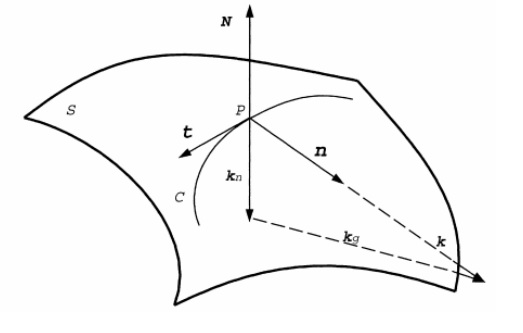
\includegraphics[width=0.6\textwidth]{Vector_Normal.jpg}
\label{fig:vectores}
\end{figure}


$\vec{k_n}$ es el vector normal de curvatura, y $\vec{k_g}$ es el vector de curvatura geodesica. Este par de vectores, son las componentes del vector de curvatura $\vec{k}$ de C. 
\begin{align} 
 \vec{k} = \frac{dt}{ds} = k \cdot \hat{n} = \vec{k_n} + \vec{k_g}, \label{eq1tangente}
\end{align}

M\'as all\'a del problema intuitivo, se toma la definici\'on formal de curva geod\'esica como la del texto sugerido en el curso.

\begin{defn}
Las curvas geod\'esicas, son aquellas que su curvatura geod\'esica es 0.
\end{defn}

De ella, se observa que no est\'a en juego la distancia entre dos puntos, y ese es el enfoque del presente trabajo. Al referirse a la curvatura geod\'esica, se refiere al valor del vector $\vec{k_g}$.


Para conocer las ecuaciones diferenciales que rigen a esta curva, se toma en cuenta la parametrizaci\'on de la superficie como $r=r(u,v)$. Siendo en realidad, $u=u(t)$ y $v=v(t)$. La $primera$ $forma$ $fundamental$ está definida por:

$$I = {ds}^2 = dr.dr = E{du}2 + 2Fdudv + G{dv}^2$$



Donde sus coeficientes son:

\begin{align} 
E = r_u . r_u \\ 
F = r_u . r_v \\ 
G = r_v . r_v 
\label{eq_coeficientes}
\end{align}


Quedando definidos $\hat{N}$ el vector unitario normal a $S$ en $P$, y $\hat{u}$ el vector unitario perpendicular a $\hat{t}$ en el plano tangente a la suferficie. Queda determiando  $\hat{u} = \hat{N} x \hat{t} $.


    La compontente $\hat{u}$ en el vector de curvatura $\hat{k}$ de 
    $r(t)$, es la curvatura geodesica $k_g$ y est\'a dada por la siguiente ecuaci\'on.

\begin{align} 
k_g = (k.\hat{u})\hat{u}
 \label{eqcurvatura_k_g}
\end{align}

La funci\'on escalar

\begin{align} 
k_g = (k.\hat{u})
 \label{eqcurvatura_kg}
\end{align}
es llamada curvatura geod\'esica de $C$ en $P$.
O, equivalentemente:

\begin{align} 
k_g = \frac{dt}{ds} . (N x t)
 \label{eqcurvatura_kg_vectores}
\end{align}

El vector tangente unitario, a la curva C puede obtenerse derivando la ecuacion param\'etrica respecto al arco, usando la siguiente relacion:

\begin{align} 
t = \frac{d r(u(s), v(d))}{ds}&=r_u \frac{d u}{ds} + r_v \frac{d v}{ds}
 \label{equ_t}
\end{align}

Por lo que se obtiene:

\begin{align} 
 \frac{d t}{ds} = r_{uu} (\frac{d u}{ds})^2 +
 2 r_{uv} \frac{d u}{ds} \frac{d v}{ds}
 + r_{vv} (\frac{d v}{ds})^2 +
 r_u \frac{d^2 u}{ds^2} +
 r_v \frac{d^2 v}{ds^2}
 \label{equ_dt}
\end{align}

en este sentido, sustituyendo en \ref{eqcurvatura_kg_vectores} los resultado de \ref{equ_t} y \ref{equ_dt}:

\begin{align} 
\begin{split}
k_g = [ 
(r_u x r_{uu}) (\frac{d u}{ds})^3 + 
(2 r_u x r_{uv} + r_v + r_{uu} ) (\frac{d u}{ds})^2 \frac{dv}{ds} + \\
(r_u x r_{vv} + 2 r_v + r_{uv})  \frac{d u}{ds} (\frac{d v}{ds})^2 + 
(r_v x r_{vv}) (\frac{d u}{ds})^3
] . N + \\
(r_u x r_{v}) . N (\frac{d u}{ds} \frac{d^2 v}{ds^2} - \frac{d^ 2 u}{ds^2 } \frac{d v}{ds})
\label{curvatura_conR}
\end{split}
\end{align}
Paraboloide 
Se observa que los coeficientes de $(\frac{d u}{ds})^3$, 
$(\frac{d u}{ds})^2 \frac{d v}{ds}$, $\frac{d u}{ds} (\frac{d v}{ds})^2$,  
$(\frac{d v}{ds})^3$,
$(\frac{d u}{ds} \frac{d^2 v}{ds^2} - \frac{d^2 u}{ds^2} \frac{d v}{ds} ) $
son todos funciones de los coeficientes definidos en \ref{eqE}-\ref{eqG} y de sus derivadas redpecto a u y v. Es interesante notar que la curvatura geodesica depende solamente de la primera forma fundamental.

Usando los s\'imbolos de Christoffel $\Gamma_{jk}^i (i,j,k=1,2)$ definidos de la siguiente forma:

\begin{align} 
\Gamma_{11}^1 = \frac{GE_u - 2 FF_u + FE_v}{2(EG - F^2)} \label{Gam_11_1}\\
\Gamma_{11}^2 = \frac{2EF_u - EE_v + FE_u}{2(EG - F^2)}\label{Gam_11_2}\\
\Gamma_{12}^1 = \frac{GE_v - FG_u}{2(EG - F^2)} \label{Gam_12_1}\\
\Gamma_{12}^2 = \frac{EG_u - FE_v}{2(EG - F^2)}\label{Gam_12_2}\\
\Gamma_{22}^1 = \frac{2GF_v - GG_u + FG_v}{2(EG - F^2)} \label{Gam_22_1}\\
\Gamma_{22}^2 = \frac{EG_u - FE_v}{2(EG - F^2)}\label{Gam_22_2}
\end{align}


la curvatura geod\'esica se reduce a:

\begin{align} 
\begin{split}
k_g = [ \Gamma_{11}^2 (\frac{du}{ds})^3 + (2 \Gamma_{12}^2 -  \Gamma_{11}^1 ) (\frac{du}{ds})^2 \frac{dv}{ds} +\\ (\Gamma_{22}^2 -  2 \Gamma_{12}^1 ) \frac{du}{ds} (\frac{dv}{ds})^2 - \Gamma_{22}^1 (\frac{dv}{ds})^3 +\\ \frac{du}{ds} \frac{d^2v}{ds^2} - \frac{d^2u}{ds^2} \frac{dv}{ds}] \sqrt(EG - F^2)
\label{eqCurvatura}
\end{split}
\end{align}

Acorde a la definici\'on, se puede determinar la ecuaci\'on diferencial de calquier geod\'esica de cualquier superficie simplemente exigiendo que el valor $k_g = 0$. Al imponer esto en la ecuaci\'on \ref{eqCurvatura} se obtiene:

\begin{align} 
\frac{du}{ds} \frac{d^2v}{ds^2} - \frac{d^2u}{ds^2} \frac{dv}{ds} = -  \Gamma_{11}^2 (\frac{du}{ds})^3 - (2 \Gamma_{12}^2 -  \Gamma_{11}^1 ) (\frac{du}{ds})^2 \frac{dv}{ds} + (2 \Gamma_{12}^1 - \Gamma_{22}^2) \frac{du}{ds} (\frac{dv}{ds})^2 + \Gamma_{22}^1 (\frac{dv}{ds})^3
\label{eqCurvatura}
\end{align}

Alternativamente, se puede derivar la ecuacion diferencial de la geodesica considerando que la superficie normal N tiene la direccion normal a la curva geodesica $+- n$.

\begin{align} 
n r_u = 0, n r_v = 0
\label{equcurvatura_nr}
\end{align}.

Mientras $kn = \frac{dt}{ds} $, la ecuacion 
\ref{equcurvatura_nr} 
puede ser escrita de la forma:

\begin{align} 
\frac{dt}{ds} r_u &=0,\frac{dt}{ds} r_v &=0
\label{equdt_ru_rv}
\end{align}

Si se sustituye en la ecuacion \ref{equdt_ru_rv} en la \ref{equ_dt} se tiene:

\begin{align} 
(r_{uu} r_u) (\frac{du}{ds})^2 + 2 (r_{uv} r_u) \frac{du}{ds} \frac{dv}{ds} + (r_{vv} r_u) (\frac{dv}{ds})^2 + E \frac{d^2u}{ds^2} + F \frac{d^2v}{ds^2} = 0
\label{equ_dt_EF}
\end{align}


\begin{align} 
(r_{uu} r_v) (\frac{du}{ds})^2 + 2 (r_{uv} r_v) \frac{du}{ds} \frac{dv}{ds} + (r_{vv} r_v) (\frac{dv}{ds})^2 + F \frac{d^2u}{ds^2} + G \frac{d^2v}{ds^2} = 0
\label{equ_dt_FG}
\end{align}

Al eliminar el t\'ermino $\frac{d^2v}{ds^2}$ de \ref{equ_dt_EF}, usando \ref{equ_dt_FG}, y eliminando en \label{equ_dt_FG} usando \label{equ_dt_EF}, empleando los s\'imbolos de Christoffel, se obtiene:

\begin{align} 
\frac{du}{ds}&=p, \label{equ1_Geo}\\
\frac{dv}{ds}&=q, \label{equ2_Geo}
\end{align}

Las ecuaciones \label{equ1_Geo} y \label{equ2_Geo} est\'am relacionanadas por la primera forma fundamental, $ds^2 = E ds^2+ 2 Fdudv+ G dv^2$. Si se elimina el termino $ds$ de ambas ecuaciones, estas ecuaciones se reducen a la \ref{eqCurvatura}


\begin{align} 
\frac{du}{ds}&=p, \label{eq1Geodesica}\\
\frac{dv}{ds}&=q, \label{eq2Geodesica}    \\
\frac{dp}{ds}&= - \Gamma_{11}^1 p^2 -2 \Gamma_{12}^1 pq - \Gamma_{22}^1 q^2, \label{eq3Geodesica}\\ 
\frac{dp}{ds}&=- \Gamma_{11}^2 p^2 -2 \Gamma_{12}^2 pq - \Gamma_{22}^2 q^2. \label{eq4Geodesica}
\end{align}

%-------------------------------------------------------------------------------
\subsection{C\'alculo de las ecuaciones en superficie param\'etrica}
En pos de reforzar el entendimiento del lector sobre el problema se presentan algunos ejemplos de superficies y sus respectivos sistemas de ecuaciones diferenciales que determinan las curvas geod\'esicas.

% PLANO
\subsubsection{Plano por el origen}
Sean $V_1=(x_1,y_1,z_1)$ y $V_2=(x_2,y_2,z_2)$ los vectores que generan el plano.
La ecuaci\'on param\'etrica \ref{planoEq} representa dicho plano.

\begin{equation} \label{planoEq}
r(u,v) = (x_1 u + x_2 v, y_1 u + y_2 v, z_1 u + z_2 v)
\end{equation}

Utilizando las ecuaciones de la geod\'esica \ref{eq1Geodesica}-\ref{eq4Geodesica}, las ecuaciones de la primera forma fundamental \ref{eqE}-\ref{eqG} y la ecuaci\'on parametrica \ref{planoEq} del plano obtenemos E, F y G en \ref{fffPlano}  y en \ref{fffuPlano}-\ref{fffvPlano} sus respectivas derivadas parciales.

\begin{align} 
E&=x_1^2 + y_1^2 + z_1^2,   & F &=x_1 x_2 + y_1 y_2 + z_1 z_2,   & G&=x_2^2 + y_2^2 + z_2^2, \label{fffPlano} \\
E_u&=0,     & F_u&=0,   & G_u&=0, \label{fffuPlano}\\
E_v&=0,    & F_v&=0,   & G_v&=0, \label{fffvPlano}
\end{align}

Entonces, como todas las derivadas parciales son nulas, usando \ref{Gam_11_1}-\ref{Gam_22_2}, los s\'imbolos de Christoffel valen cero.

Finalmente obtenemos las ecuaciones de la geod\'esica para el plano en \ref{eq:duPlano}-\ref{eq:dqPlano}.

\begin{align}
\frac{du}{ds}&=p,\label{eq:duPlano} \\
\frac{dv}{ds}&=q,\label{eq:dvPlano}     \\
\frac{dp}{ds}&=0, \label{eq:dpPlano}\\ 
\frac{dq}{ds}&=0 \label{eq:dqPlano}
\end{align}

% ESFERA
\subsubsection{Esfera unitaria centrada en el origen}

La ecuaci\'on param\'etrica \ref{esferaEq} representa una esfera unitaria centrada en el origen.
\begin{equation} \label{esferaEq}
r(u,v) = (cos (u) sin(v), sin (u) sin (v),cos (v)), \\
(u,v) \in  [o, 2 \pi] \times [0, \pi]
\end{equation}
De forma an\'aloga que el caso anterior, utilizamos las ecuaciones de la geod\'esica \ref{eq1Geodesica}-\ref{eq4Geodesica}, las ecuaciones de la primera forma fundamental \ref{eqE}-\ref{eqG} y la ecuaci\'on parametrica \ref{esferaEq} del plano obtenemos E, F y G en \ref{fffEsfera} las ecuaciones de la primera forma fundamental y en \ref{fffuEsfera}-\ref{fffvEsfera} sus respectivas derivadas parciales.

\begin{align}
E&=sin^2 (v),   & F &=0    & G&=1, \label{fffEsfera} \\
E_u&=0,     & F_u&=0,   & G_u&=0, \label{fffuEsfera}\\
E_v&=2sin(v)cos(v),    & F_v&=0,   & G_v&=0, \label{fffvEsfera}
\end{align}

De esta forma, usando \ref{Gam_11_1}-\ref{Gam_22_2}, obtenemos los s\'imbolos de Christoffel en \ref{CS1Esfera}-\ref{CS3Esfera}

\begin{align}
\Gamma_{12}^2&=\Gamma_{11}^1=\Gamma_{22}^1=\Gamma_{22}^2=0, \label{CS1Esfera} \\
\Gamma_{12}^1&=\frac{cos(v)}{sen(v)},  \label{CS2Esfera}   \\
\Gamma_{11}^2&=-sen(v)cos(v) .  \label{CS3Esfera}
\end{align}

Las ecuaciones de la geod\'esica para la esfera son \ref{eq:duEsfera}-\ref{eq:dqEsfera}.

\begin{align}
\frac{du}{ds}&=p,\label{eq:duEsfera} \\
\frac{dv}{ds}&=q,\label{eq:dvEsfera}     \\
\frac{dp}{ds}&=\frac{-2cos(v)}{sen(v)} pq, \label{eq:dpEsfera}\\ 
\frac{dq}{ds}&= sen(v)cos(v) p^2. \label{eq:dqEsfera}
\end{align}

%-------------------------------------------------------------------------------
%PARABOLOIDE HIPERBOLICO
\subsubsection{Paraboloide hiperb\'olico}

La ecuaci\'on param\'etrica \ref{parHipEq} representa el paraboloide hiperb\'olico.
\begin{equation} \label{parHipEq}
r(u,v) = (u,v,uv)
\end{equation}

Nuevamente, a partir de las ecuaciones de la geod\'esica \ref{eq1Geodesica}-\ref{eq4Geodesica}, las ecuaciones de la primera forma fundamental \ref{eqE}-\ref{eqG} y la ecuaci\'on parametrica \ref{parHipEq} del plano obtenemos E, F y G en \ref{fffHipEq} las ecuaciones de la primera forma fundamental y en \ref{fffuHipEq}-\ref{fffvHipEq} sus respectivas derivadas parciales.

\begin{align}
E&=1+v^2,   & F &=uv    & G&=1+u^2, \label{fffHipEq} \\
E_u&=0,     & F_u&=v,   & G_u&=2u, \label{fffuHipEq}\\
E_v&=2v,    & F_v&=u,   & G_v&=0, \label{fffvHipEq}
\end{align}

A partir de lo anterior se sustituye en \ref{Gam_11_1}-\ref{Gam_22_2} y se obtienen los s\'imbolos de Christoffel en \ref{CS1HipEq}-\ref{CS3HipEq}.

\begin{align}
\Gamma_{11}^1&=\Gamma_{11}^2=\Gamma_{22}^1=\Gamma_{22}^2=0, \label{CS1HipEq} \\
\Gamma_{12}^1&=\frac{v}{u^2+v^2+1},  \label{CS2HipEq}   \\
\Gamma_{12}^2&=\frac{u}{u^2+v^2+1}.  \label{CS3HipEq}
\end{align}

Las ecuaciones de la geod\'esica para el paraboloide hiperb\'olico son \ref{eq:du}-\ref{eq:dq}.

\begin{align}
\frac{du}{ds}&=p,\label{eq:du} \\
\frac{dv}{ds}&=q,\label{eq:dv}     \\
\frac{dp}{ds}&=\frac{-2v}{u^2+v^2+1} pq, \label{eq:dp}\\ 
\frac{dq}{ds}&=\frac{-2u}{u^2+v^2+1} pq. \label{eq:dq}
\end{align}


%-------------------------------------------------------------------------------
%
%-------------------------------------------------------------------------------
\section{Metodolog\'ia}\label{Metodo}
El sistema de ecuaciones diferenciales \ref{eq1Geodesica}-\ref{eq4Geodesica} puede resolverse model\'andolo de las siguientes dos formas:
\begin{itemize}
    \item Problema de Valor Inicial (PVI).
    \item Problema con Condiciones de Borde (PCB).
\end{itemize}
La primera forma consiste en proporcionar el valor inicial para cada una de las cuatro ecuaciones diferenciales del sistema.
Como la soluci\'on de un PVI es \'unica, al indicar los valores iniciales queda determinada una sola curva. \\
En el caso del PCB se dan dos puntos del espacio como condiciones de borde por lo que las ecuaciones diferenciales del sistema tienen muchas soluciones o incluso ninguna. \\

Generalmente problema a resolver se asemeja a un PCB que a un PVI, por lo que la forma m\'as natural de resolverlo ser\'ia a partir del segundo. Debido a que la complejidad computacional que implica el PCB es considerablemente mayor que el PVI se opt\'o por el primer m\'etodo para la resoluci\'on. En ~\ref{PVI} se demuestra que es posible modelar las geod\'esicas como un PVI. \\

Por otro lado el sistema presentado en \ref{eq1Geodesica}-\ref{eq4Geodesica} es un sistema anal\'itico y no puede resolverse computacionalmente por lo que es necesario utilizar un algoritmo num\'erico para para modelar y aproximar el problema. El m\'etodo seleccionado para el estudio del fue el m\'etodo de Euler hacia adelante, que fue elegido debido a su simplicidad en comparaci\'on a otros m\'etodos considerados como el M\'etodo del Trapecio.


%-------------------------------------------------------------------------------
%INICIO SECCION 3.1
%-------------------------------------------------------------------------------
\subsection{Problema de Valor Inicial (PVI)}\label{PVI}

El Problema de Valor Inicial, tambi\'en conocido como problema de Cauchy, es b\'asicamente un sistema de ecuaciones compuesto de una EDO y una condici\'on inicial de la misma. \\

A continuaci\'on se explica en m\'as detalle y demuestra que las geod\'esicas en el paraboloide hiperb\'olico es un PVI. \\

Previamente, se extraen de  REFLIBROCURSO las siguientes definiciones que nos ayudaran en la muestra:

\begin{itemize}
    \item Una ecuaci\'on diferencial es una ecuaci\'on que relaciona las derivadas de una o m\'as variables dependientes respecto a una o m\'as variables independientes.
    \item Una ecuaci\'on diferencial ordinaria (EDO) es una ecuaci\'on diferencial que relaciona una funci\'on desconocida de una \'unica variable independiente con sus derivadas.
    \item Dada una funci\'on $f: R^2 \rightarrow R $el Problema de Valores Iniciales consiste en hallar la funci\'on $y = y(x)$ tal que:
    \end{itemize}
$$(P V I):
        \left \{
          \begin{tabular}{c}
          $y'(x) = f(x,y(x))$ \\
          $y(x_0) = y(y_0) \in R$\\
          \end{tabular}
        \right.$$
    % No es necesario
    %Por ejemplo, si $y' = x^2y+2y \rightarrow f(x,y(x)) = x^2y+2y $
    
    
 %   Entonces considerando las ecuciones planteadas en  \ref{eq:du} - \ref{eq:dq}  del paraboloide hiperb\'olico.
    
% No va, basta con referenciar las originales
%\begin{align}
%\frac{du}{ds}&=p,\label{eq:du} \\
%\frac{dv}{ds}&=q,\label{eq:dv}     \\
%\frac{dp}{ds}&=\frac{-2v}{u^2+v^2+1} pq, \label{eq:dp}\\ 
%\frac{dq}{ds}&=\frac{-2u}{u^2+v^2+1} pq. \label{eq:dq}
%\end{align}          
 
Entonces utilizando las ecuaciones planteadas en  \ref{eq:dupvi} - \ref{eq:dqpvi}  del paraboloide hiperb\'olico y considerando la siguiente notaci\'on:

\begin{align}
u'(s)=\frac{du}{ds}&=p &\rightarrow u'(s) = f_1 (s,u(s)) ,\label{eq:dupvi} \\
v'(s)=\frac{dv}{ds}&=q &\rightarrow v'(s) =f_2 (s,v(s)),\label{eq:dvpvi}     \\
p'(s)=\frac{dp}{ds}&=\frac{-2v}{u^2+v^2+1} pq &\rightarrow p'(s)=f_3 (s,p(s)), \label{eq:dppvi}\\ 
q'(s)=\frac{dq}{ds}&=\frac{-2u}{u^2+v^2+1} pq &\rightarrow q'(s)=f_4 (s,p(s)). \label{eq:dqpvi}
\end{align}

se puede representar las ecuaciones diferenciales como un PVI de la siguiente manera:

$$(P V I):
        \left \{
          \begin{tabular}{c}
            $y'(s)= \vec{f}(s,u(s),v(s),p(s),q(s))$\\
            $y(s_0) = (u(s_0),v(s_0),p(s_0),q(s_0)) \in R^4$\\
          \end{tabular}
        \right.$$



%-------------------------------------------------------------------------------
%FIN SECCION 3.1
%-------------------------------------------------------------------------------




\subsection{Discretizaci\'on del problema}\label{sec:disc}

Para la discretizacion del problema de valores iniciales se utiliza el metodo de Euler, denominado en honor a su autor Leonhard Euler. Este algoritmo es elegido por su simplicidad.

%Como m\'etodo de primer orden el error local es proporcional al cuadrado del paso, y el error global es proporcional al paso.\\

Este metodo tiene dos variantes Euler hacia Adelante y Euler hacia Atras partiendo de las ecuaciones (\ref{eq:du}-\ref{eq:dq}) se aplica el M\'etodo de Euler hacia Adelante. A continuaci\'on se calculan las ecuaciones en su forma discreta.\\

%En este trabajo se limitó al analisis de las geodesicas sobre paraboloide hiperbolico pero el razonamiento puede deducirse analogamente para otras superficies. 


Primero realizamos el c\'alculo para $u$:\\
$$\frac{du}{ds}=p \Rightarrow \frac{u_{k+1}-u_k}{h}=p_k \Rightarrow u_{k+1}=u_k+p_k h $$\\
Para $v$:\\
$$\frac{dv}{ds}=q \Rightarrow \frac{v_{k+1}-v_k}{h}=q_k \Rightarrow v_{k+1}=v_k+q_k h $$\\
Para $p$:\\
$$\frac{dp}{ds}=\frac{-2v}{u^2+v^2+1} pq \Rightarrow \frac{p_{k+1}-p_k}{h}=\frac{-2v_k}{u_k^2+v_k^2+1} p_kq_k \Rightarrow p_{k+1}=\frac{-2v_k }{u_k^2+v_k^2+1} p_kq_k h + p_k $$\\
Finalmente, para $q$:\\
$$ \frac{dq}{ds}=\frac{-2u}{u^2+v^2+1} pq \Rightarrow \frac{q_{k+1}-q_k}{h}=\frac{-2u_k}{u_k^2+v_k^2+1} p_kq_k \Rightarrow q_{k+1}=\frac{-2u_k}{u_k^2+v_k^2+1} p_kq_k h +q_k $$\\


En resumen:
\begin{align}
u_{k+1}&=u_k+p_k h \label{eq:dudis} \\
v_{k+1}&=v_k+q_k h \label{eq:dvdis} \\
p_{k+1}&=\frac{-2v_k }{u_k^2+v_k^2+1} p_kq_k h + p_k \label{eq:dpdis} \\
q_{k+1}&=\frac{-2u_k}{u_k^2+v_k^2+1} p_kq_k h +q_k\label{eq:dqdis}
\end{align}

El  siguiente pseudoc\'odigo \ref{pscod:euler} expresa una forma de introducir el problema en softwares tales como "Octave", "R", "Python", etc.

\begin{algorithm}
  \caption{Pseudoc\'odigo para resolver y graficar el PVI mediante el m\'etodo "Euler hacia adelante"}
    \label{pscod:euler}
  \begin{algorithmic}[1]
  \Require{ $y(0) = y0 ; x(0) = 0; i = 1; h; f$}
%  \Statex
  \While {$x(i) < x(f) $}
  \State $\textit{y(i+1)} \gets \text{length of }\textit{y(i) + h ∗ f (x(i), y(i))}$
  \State $\textit{x(i + 1)} \gets x(i) + h$ 
  \State$i\gets\i+1$
   \EndWhile
  \end{algorithmic}
\end{algorithm}


%-------------------------------------------------------------------------------
%
%-------------------------------------------------------------------------------
\section{Estudio Experimental}\label{Resultados}
\subsection{Ambiente de trabajo}\label{ambiente}
Durante el desarrollo de la experiencia se trabajo con:
\begin{itemize}
    \item Lenguaje de programaci\'on: Octave.
    \item Caracter\'isticas de la computadara utilizada:
    \begin{itemize}
        \item HP Pavilion 15 Notebook
        \item Procesador:AMD A10-7300 Radeon R6, 10 Compute Cores 4C+6G
        \item Memoria RAM: 8 GB
        \item Sistema Operativo: Manjaro 17.1.12 x64 (Deepin desktop)
        \item Versión de Octave: 4.4.1
        \item Epsilon de m\'aquina: $2.2204x10^{-16}$
    \end{itemize}
\end{itemize}


\subsection{Resultados Obtenidos}
Utilizando el ambiente de desarrollo descrito en la secci\'on \ref{ambiente}, fueron ejecutados los scripts realizados \cite{scripts}.
En la Fig. \ref{ph} se despliega la curva geod\'esica bajo las siguiente condiciones:
\begin{itemize}
    \item Valores iniciales: $u=4$, $v=1$, $p=1$ y $q=1$.
    \item Paso: $h=0.1$.
    \item N\'umero m\'aximo de iteraciones $max\_it=101$.
\end{itemize}
Se puede observar que en este caso, ambas curvas van sobre la superfice del paraboloide. Así como tabi\'en 

\begin{figure}[H]
\caption{Paraboloide Hiperb\'olico}
\centering
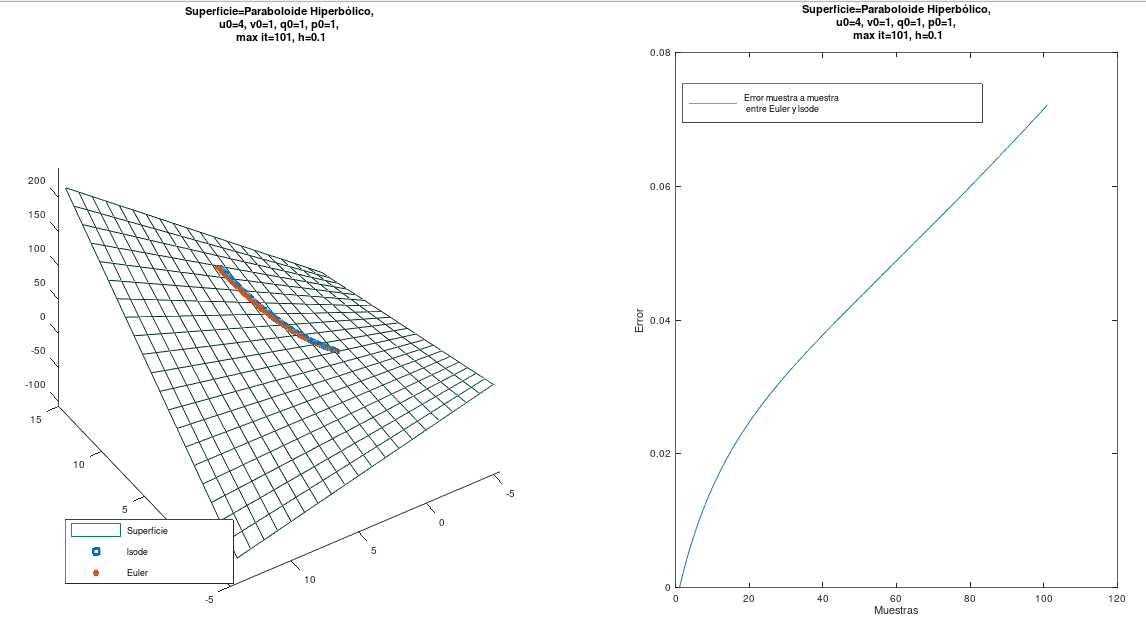
\includegraphics[width=0.9\textwidth]{ph.png}
\label{ph}
\end{figure}


Por otro lado, en la Fig.\ref{phmal} se utilizaron las siguientes caracter\'isticas:
\begin{itemize}
    \item Valores iniciales: $u=4$, $v=1$, $p=1$ y $q=1$.
    \item Paso: $h=1$.
    \item N\'umero m\'aximo de iteraciones $m=101$.
\end{itemize}


\begin{figure}[H]
\caption{Paraboloide Hiperb\'olico}
\centering
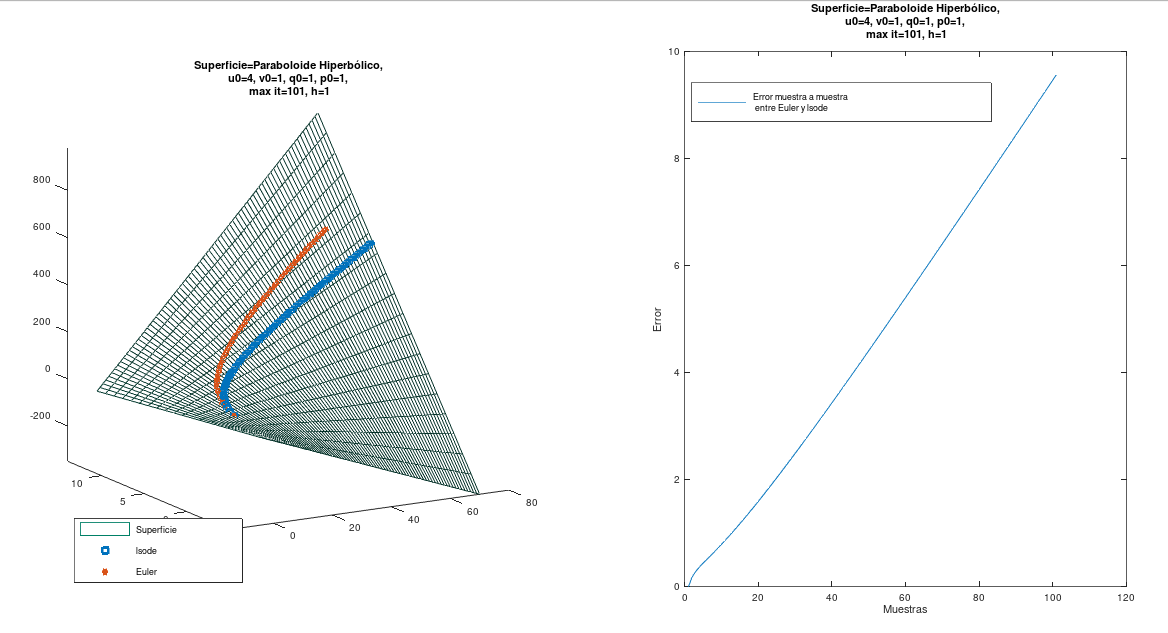
\includegraphics[width=0.9\textwidth]{phmal.png}
\label{phmal}
\end{figure}

%-------------------------------------------------------------------------------
%
%-------------------------------------------------------------------------------
\section{Conclusiones}\label{Conclusiones}


En este trabajo se intentó analizar de manera practica la generacion de curvas geodesicas definidas sobre diferentes superficies parametrizadas por longitud de arco mediante el metodo numerico de Euler tal como lo define el Instituto de Matematica y Estadistica Rafael Laguardia en las notas del curso de Metodos Numericos (insert cita). Este analisis fue realizado desde un punto de vista experimental enfocado en entender el funcionamiento y comportamiento de la estimacion de ecuaciones diferenciales mediante metodos numericos, los hallazgos identificados son 

Al considerar las geod\'esicas como un Problema de Valor Inicial se simplifica el modelo y se reduce la dificultad del algoritmo num\'erico que lo resuelve. Si bien el trabajo realizado cumple con el objetivo, encontrar una aproximaci\'on a la curva geod\'esica que pasa por un punto inicial est\'a lejos de resolver el problema real que es encontrar la distancia minima entre dos puntos de una superficie.  Por lo que como trabajo a futuro se recomienda abordar el problema de las geod\'esicas como un Problema de Condiciones de Borde.


%-------------------------------------------------------------------------------

%\section*{Acknowledgment}
%This work is partially supported by Project CSIC I+D 395 entitled \emph{Sistemas Binarios
%Estoc\'asticos Din\'amicos}.


\bibliographystyle{plain}
%\bibliographystyle{endm.bst}
\bibliography{biblio}

\newpage

\section*{Anexos}

\subsection*{Curvas geod\'esicas del plano y la esfera}
En la secci\'on \ref{sec:disc} se discretiz\'o las ecuaciones diferenciales que caracterizan las geod\'esicas en el paraboloide hiperb\'olico utilizando el m\'etodo de "Euler hacia adelante". En esta secci\'on se mostrar\'a como quedan las mismas para un plano y para una esfera. Tambi\'en se mostrar\'an dos ejemplos gr\'aficos para cada caso. En \'estos se comparar\'an dos m\'etodos num\'ericos, el anteriormente dicho y el implementado por octave en la funci\'on "lsode".

El caso del plano, la curva geod\'esica es un segmento de recta. Entre los dos puntos correspondientes a un paso, la distancia para el método de Euler es el valor del paso por el vector dirreci\'on. \'Esta simpleza produce que la diferencia entre ambos m\'etodos sea nula al tabajar con 10 pasos (Fig. \ref{fig:plano}), o cuasi nula trabajando con 100 pasos (Fig. \ref{fig:planoh100} y Fig.\ref{fig:planoh100q03})ya que es 14 ordenes inferior al valor del paso (el m\'aximo error obtenido en \'esta curva fue inferior a $4x10^{-12}$ con un paso de 100).
\begin{figure}[H]
\caption{Plano: Sin diferencia apreciable entre ambos m\'etodos}
\centering
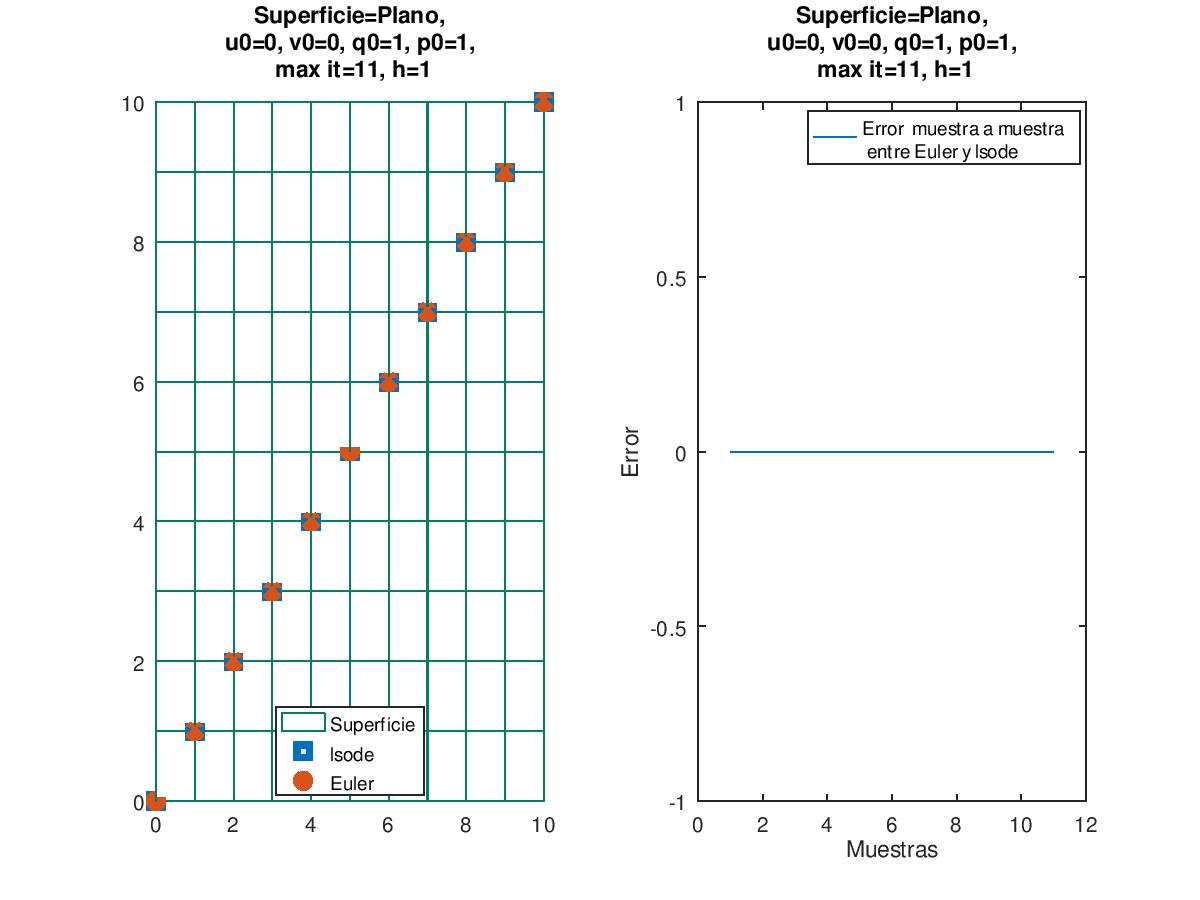
\includegraphics[width=0.5\textwidth]{plano.jpg}
\label{fig:plano}
\end{figure}

\begin{figure}[H]
\caption{Plano: Diferencia apreciable entre ambos m\'etodos }
\centering
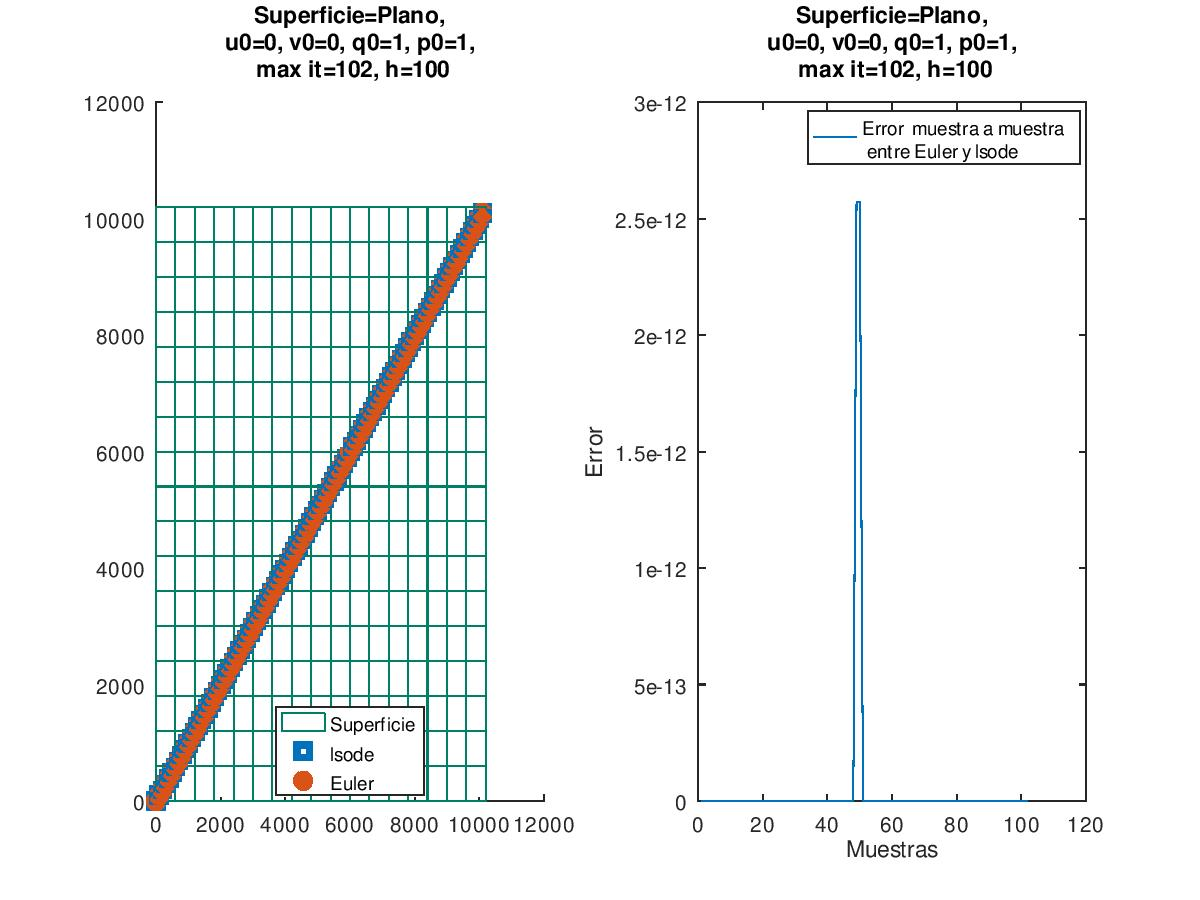
\includegraphics[width=0.5\textwidth]{planoh100.jpg}
\label{fig:planoh100}
\end{figure}

\begin{figure}[H]
\caption{Plano: Diferencia apreciable entre ambos m\'etodos }
\centering
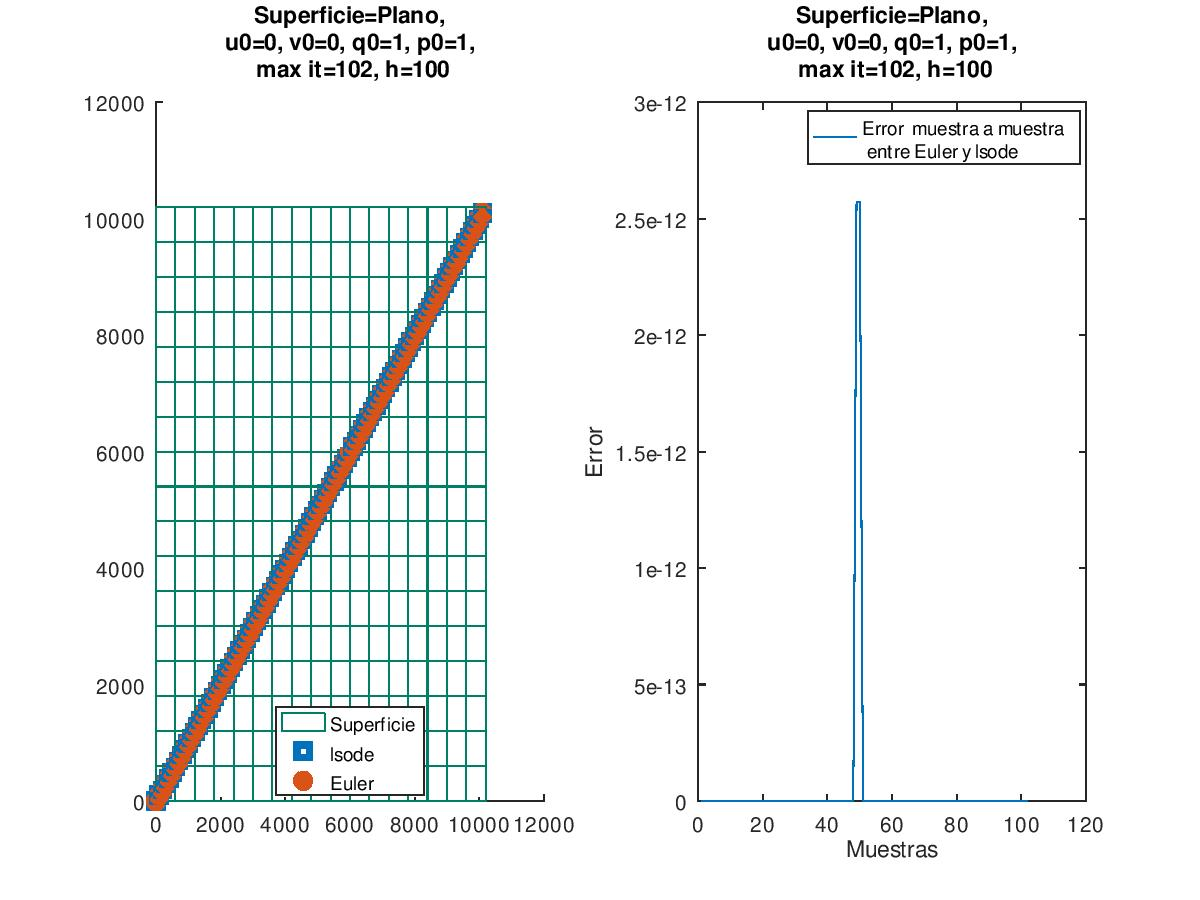
\includegraphics[width=0.5\textwidth]{planoh100.jpg}
\label{fig:planoh100q03}
\end{figure}



\begin{figure}[H]
\caption{Esfera: Sin diferencia apreciable entre ambos m\'etodos}
\centering
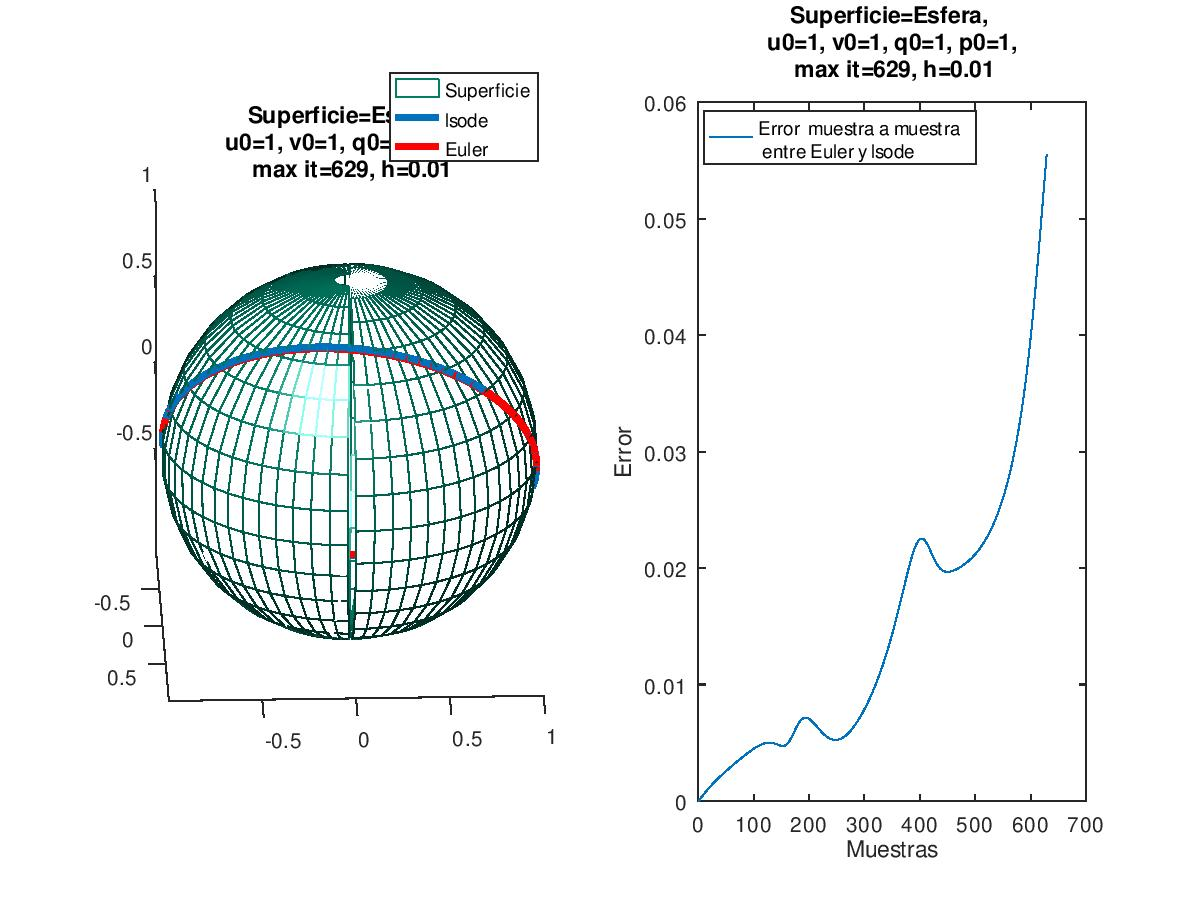
\includegraphics[width=0.5\textwidth]{esfera.jpg}
\label{fig:esfera}
\end{figure}

\begin{figure}[H]
\caption{Esfera: Diferencia apreciable entre ambos m\'etodos }
\centering
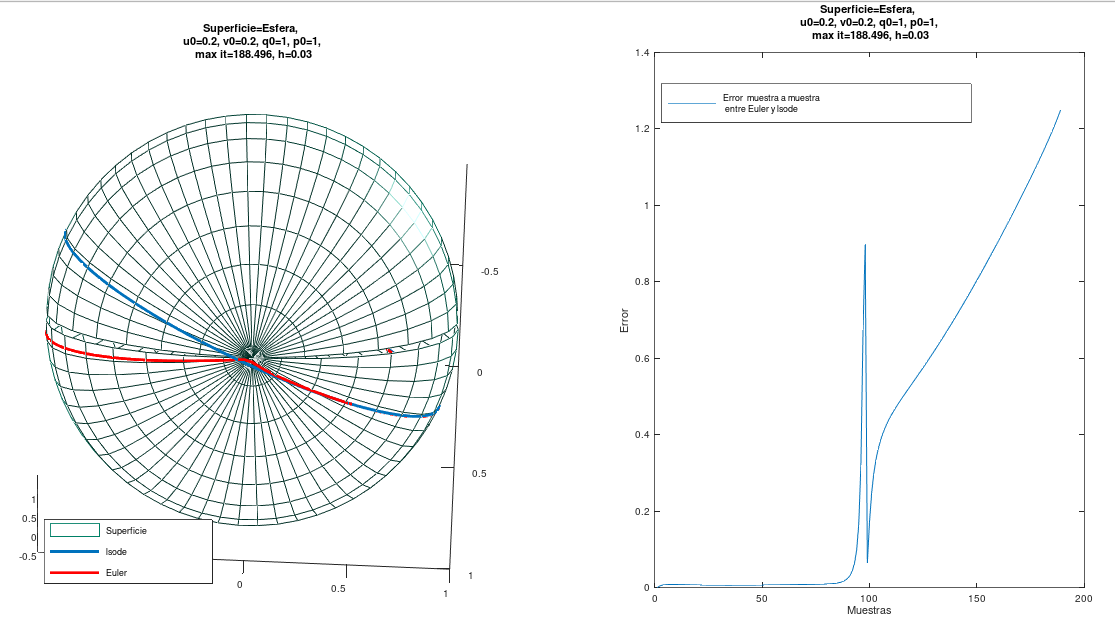
\includegraphics[width=0.5\textwidth]{esferarara.png}
\label{fig:esferamal}
\end{figure}


\tableofcontents


\end{document}
